\chapter{Convección Mixta En Transición Laminar-Turbulenta} \label{cap:transicion}

El en presente capítulo se examina la transición laminar-turbulenta en convección mixta en un canal de placas paralelas mediante simulaciones DNS. El mismo se organiza en tres partes: (i) la exploración de distintas condiciones iniciales mediante la evolución temporal de magnitudes de interés (TKE y Re$_{\tau}$) contemplando dos valores del número de Richardson Re$_b$ (casos A y B); (ii) un análisis detallado del caso correspondiente al Ri$_b$ más bajo simulado, cuya perturbación emplea una combinación de ondas 2D/3D (ensayo A-C10); (iii) un análisis detallado del caso correspondiente al Ri$_b$ más alto simulado, cuya perturbación emplea únicamente una onda 2D (ensayo B-C2). %Este ordenamiento permite evaluar la sensibilidad del proceso de transición según la naturaleza de la perturbación inicial empleada y comparar la dinámica de transición bajo diferentes intensidades de fuerza boyante.

En los ensayos A-C10 y B-C2 se consideran las siguientes magnitudes de interés: la energía cinética turbulenta (TKE) y la varianza de la temperatura adimensional; perfiles de velocidad y de temperatura adimensional en instantes representativos; el factor de fricción de Darcy y número de Nusselt. Este conjunto de métricas permite vincular la dinámica de la transición con su impacto termo-hidrodinámico y con el acercamiento a los estados de referencia de convección mixta completamente desarrollada.

En los ensayos con Ri$_b$ más bajo ($\text{Ri}_b=0\text{.}04$) se requirió emplear una combinación de perturbaciones bidimensionales y tridimensionales para desencadenar la transición. Por su parte, aquellos ensayos con Ri$_b$ más alto ($\text{Ri}_b=1\text{.}06$), si bien también se consideraron condiciones iniciales construidas con combinaciones de ondas 2D/3D, fue posible inestabilizar el flujo empleando únicamente ondas 2D. 

En el ensayo A-C10, en un etapa inicial ($t^*\lesssim 400$), la evolución temporal de las cantidades se caracteriza por experimentar valles y máximos locales y absolutos, salvo en número de Nusselt que en esta estapa se mantiene practicamente constante. Luego, estas magnitudes tienden hacia el estado de referencia estadísticamente estacionario. En particular, las cantidades asociadas al aspecto hidrodinámico del sistema evoluciónan a mayor ritmo respecto de aquellas cantidades asociadas al aspecto térmico. Al inspeccionar los perfiles de velocidad y temperatura es posible apreciar una pérdida de simetría; mediante un análisis cualitativo de las estructuras de vórtices es posible dar cierto entendimiento de esta cuestión.  

Por otro lado, en el ensayo B-C2, las magnitudes de interés experimentan un breve período laminar y luego tienen un crecimiento brusco, salvo el número Nusselt que decrece. Esta cuestión, ocurre para los instantes de tiempo tales que $t^*\lesssim 50$. En tiempos posteriores, luego de experimentar esa subida, las cantidades decaen y convergen hacia el estado desarrollado con la excepción de Nu que tiende a recupersarse de su mínimo, pero sin alcanzar el valor de referencia del estado estadísticamente estacionario. 

Al comparar los ensayos A-C10 y B-C2, se observa que el incremento de la fuerza boyante acelera la transición: los picos (máximos absolutos) aparecen antes y el paso del régimen laminar al turbulento ocurre en menor tiempo.

\newpage

\section{Exploración de casos}

Como se menciona en los Capítulos \ref{cap:intro} y \ref{cap:modelo}, la convección mixta en canales ha sido investigada exhaustivamente debido a sus múltiples aplicaciones de interés. Sin embargo, la transición laminar-turbulenta en convección mixta apenas ha sido objeto de investigación. En la bibliografía reciente existen escasos trabajos, uno de ellos es el de Chen y Chung \cite{chen2003direct}, donde se analiza el fenómeno de transición temporal.

Por esta razón, se realiza primero una exploración numérica que permita identificar combinaciones de perturbaciones capaces de inducir la inestabilidad del flujo. Se seleccionan dos números de Richardson \textit{bulk} que corresponden a soluciones desarrolladas con diferentes características: una levemente afectada por la fuerza boyante y la otra con perfiles de velocidad y temperatura claramente influidos por la flotación. Estos corresponden a los casos A y B de la Tabla \ref{tab:cases}, respectivamente, y en ambos se considera Re$_o$=5000 y Pr=0.71.

El mecanismo de inestabilización se construye a partir de condiciones iniciales de acuerdo a las ecuaciones \ref{eq:init_con_1} - \ref{eq:init_con_3} seleccionando distintos números de onda y amplitudes (véase Sección \ref{sec:mecanismo}). Los autovalores, y sus autofunciones asociadas, se obtuvieron mediante el análisis de estabilidad lineal descrito en el Capítulo \ref{cap:modelo}, utilizando la herramienta OSMC descrita en el Capítulo \ref{cap:numerico}. El espectro de autovalores y las autofunciones empleadas se encuentran disponibles en el Apéndice \ref{cap:transition_apendice}. 

Por otro lado, para decidir si una perturbación arbitraria es capaz de inestabilizar el flujo se estudia la evolución temporal de las siguientes magnitudes:

\begin{itemize}
  \item la energía cinética turbulenta, TKE o $k$, definida en el Capítulo \ref{cap:modelo}: 
  	\begin{equation*}
  		k = \frac{1}{2} \left[ \langle u^{* \prime}_x u^{* \prime}_x \rangle + \langle u^{* \prime}_y u^{* \prime}_y \rangle + \langle u^{* \prime}_z u^{* \prime}_z \rangle \right] \ 
  	\end{equation*}
  	
  

  \item y el número de Reynolds de fricción
        $$
          \text{Re}_{\tau} = \frac{u_{\tau}\,d}{\nu} ; \quad u_{\tau}= U_o \sqrt{\text{Re}_o}
        $$
        donde $u_{\tau}$ es la velocidad de fricción \cite{pope2001turbulent}.
\end{itemize}

\begin{table}[H]
\centering
\resizebox{0.24\textwidth}{!}{%
\begin{tabular}{lccc}
\toprule
Caso & Ri$_b$ & Ra \\
\midrule
A & 0.04 & 65 \\
B & 1.06 & 17750 \\
\bottomrule
\end{tabular}}
\caption{Parámetros adimensionales de los dos casos elegidos.}
\label{tab:cases}
\end{table}

\textit{\textbf{Aclaración Importante.}} En las siguientes secciones, el lector hallará gráficas con la evolución temporal de las magnitudes  Re$_{\tau}$, TKE, varianza de la temperatura, número de Nusselt (Nu) y factor de fricción de Darcy ($f$). En ellas, aparecen representados valores constantes mediante lineas a trazos cuyas etiquetas contienen los subíndices ``Init'' y ``Dev''. El primer subíndice corresponde al cálculo de las magnitudes antes mencionadas empleando los perfiles de las condiciones iniciales ($t^*=0$); el segundo corresponde al cálculo de las magnitudes empleando los perfiles del flujo turbulento completamente desarrollado, presentados en el Capítulo \ref{cap:desarrollado}. Para el cálculo de Nu y $f$ se emplea las ecuaciones \ref{eq:nu} y \ref{eq:darcy}, respectivamente.

Dado que los perfiles en $t^*=0$ son muy similares a los perfiles del flujo base laminar, los valores de Re$_{\tau}$, Nu y $f$ calculados con la condición inicial son equivalentes a los calculados en el régimen laminar. Por otro lado, los valores de TKE y la varianza de la temperatura se aproximan utilizando las autofunciones $\lbrace \widehat{v_x}, \widehat{v_y}, \widehat{v_z}, \widehat{\theta} \hspace{0.3mm} \rbrace$ que aparecen en las expresiones de las perturbaciones. Esto surge de considerar lo siguiente: 

$$\xi^{\prime} (x^*,y^*,z^*,t^* = 0) \approx \widetilde{\xi}(x^*,y^*,z^*,t^*=0) =  \widehat{\xi}(y^*) e^{i (\alpha x^* + \beta z^*)} , $$
donde $\widetilde{\xi}$ representa una perturbación arbitraria y $\widehat{\xi}$ su amplitud asociada. De esta manera, los valores de TKE y $\langle \theta^{* \prime} \theta^{* \prime} \rangle$ se estiman mediante las relaciones \ref{eq:tke-calc} y \ref{eq:varteta-calc} donde $\widetilde{\mathbf{v}}$ y $\widetilde{\varphi}$ estan dadas por las ecuaciones \ref{eq:init_con_2} y \ref{eq:init_con_3}, respectivamente.

\begin{align}
\text{TKE} &\simeq \frac{1}{2} \int \left[ \widetilde{\mathbf{v}} \cdot \widetilde{\mathbf{v}} \right] dx^* dy^* dz^* 
\label{eq:tke-calc}\\
\langle \theta^{* \prime} \theta^{* \prime} \rangle  &\simeq \int \left[ \widetilde{\varphi} \hspace{0.2mm} \right]^2 dx^* dy^* dz^* 
\label{eq:varteta-calc}
\end{align}  

%\footnote{En efecto, este cálculo se realizo. Luego, se comparó el valor calculado de estas magnitudes utilizando la condición inicial por un lado, y la solución laminar, por el otro. Los resultados arrojados son completamente consistentes.}

\subsection{Caso A (Ri$_b$=0.04)}

En la Figura \ref{fig:case-A-Re5000-Pr071} se expone la evolución en el tiempo de TKE y Re$_{\tau}$ para las distintas condiciones iniciales consideradas. Los parámetros asociados a las perturbaciones de dichas condiciones se resumen en la Tabla \ref{tab:grupo1}. Adicionalmente, se añaden los valores asociados al caso turbulento completamente desarrollado (linea a trazos roja).  

Las condiciones iniciales de los cuatro primeros ensayos, de A‑C1 a A‑C4, se construyen empleando únicamente una onda bidimensional y un mismo conjunto de autofunciones cuya parte imaginaria del autovalor ($\lambda_{2D}$=1.212 + 0.037 j) es la cota superior\footnote{Esto  se conoce como modo más inestable \cite{schmid}.} de todo el espectro de autovalores asociado. Por otro lado, se varían las amplitudes 2D utilizadas: al aumentar A$_\text{2D}$ del 1 \% al 6 \% (Tabla \ref{tab:grupo1})  no se logra gatillar la transición. En su lugar, el efecto que se logra es la traslación (adelanto) del máximo en la TKE desde $t^* \approx 140$ hasta $t^* \approx 80$. En todos los casos, luego de crecer y alcanzar un valor máximo, la TKE retorna a niveles cercanos a su valor inicial ($t^*=0$). Por su parte, los valores de Re$_{\tau}$ permanecen practicamente constante hasta $t^* \approx 100$ donde comienza un descenso de la magnitud y posteriormentes tiende a recuperarse y evolucionar, aparentemente, hacia su estado inicial. Sin embargo, como lo que se busca es una transición temprana del flujo, se opta por finalizar las simulaciones de estos ensayos.  

Por otro lado, se trata de inducir la inestabilidad empleando otras autofunciones. Se conserva la amplitud (6 \%) y se utilizan autofunciones de modos menos inestables (véase Tabla \ref{tab:grupo1} y Apéndice \ref{cap:transition_apendice}). Estos casos corresponden a los ensayos A-C7 y A-C8. En ambos, la TKE crece hasta un máximo absoluto, que continua con un segundo máximo local de menor intensidad y finaliza con una pequeña replica de aún menor intensidad (aproximadamente un órden de magnitud menor) para luego retornar a valores próximos al estado inicial. El comportamiento descrito es similar en ambos casos, con la diferencia que en el ensayo A-C7 la dinámica se retrasa respecto a la de A-C8\footnote{ Esta cuestión coincide con el hecho de que la parte imaginaria del autovalor correspondiente a A-C7 es mayor que el de A-C8.}. El restraso en la dinámica se aprecia al comparar ambos máximos absolutos: para A-C7 el máximo se encuentra en $t^* \approx 340$, mientras que para A-C8 está ubicado en  $t^* \approx 180$. Por su parte, el descenso de Re$_{\tau}$ se retrasa en ambos casos, siendo más extenso en el ensayo A-C7. Luego, en los dos ensayos, el sistema adquiere una nueva condición de flujo que, al menos hasta el tiempo simulado, es distinto del estado inicial. No obstante, no se ha encontrado indicios de que una transición temporal temprana vaya a ocurrir.  

El uso exclusivo de ondas bidimensionales resulta, aparentemente, insuficiente para desencadenar la transición del flujo. Por ello, resulta necesario buscar otra estrategia o herramienta que nos permita inestabilizar al mismo. Se procede entonces a emplear una combinación de ondas bidimensionales y tridimensionales para construir una perturbación que pueda reproducir la inestabilidad secundaria (Sección \ref{sec:mecanismo}). En este sentido, las condiciones iniciales de los ensayos A‑C9 y A‑C10 se construyen empleando la combinación de una onda 2D (A$_\text{2D}=6$ \% y mismas autofunciones de los casos A-C7 y A-C8, respectivamente) con dos ondas 3D oblicuas (A$_\text{3D}=1$ \%). 

En una primera etapa, tanto la energía cinética turbulenta como el Re$_{\tau}$ reproducen el mismo comportamiento que experimentan los ensayos A‑C7 y A‑C8. Posteriormente, para $t^* \gtrsim 395$ (A-C9) y $t^* \gtrsim 340$ (A-C10), los casos se despegan y experimentan un crecimiento brusco seguido de un pico y un ligero descenso. Luego, las magnitudes se sostienen en el tiempo en torno al valor del caso completamente desarrollado; es decir, no decaen como en los casos anteriores. Esto indica el comienzo de la transición hacia un régimen turbulento, y para estos dos ensayos simulados, se observa que la combinación de ondas 2D y 3D resulta exitosa para inestabilizar el flujo. 

\paragraph{Caso representativo.} El ensayo \textbf{A‑C10} se elige como referencia para la discusión detallada (Sección \ref{sec:ac10}) ya que se logra una transición temprana del flujo ($t^* \approx 300$) que fue claramente inducida y además que se sostiene en el tiempo ($t^*>400$). 

\begin{table}[H]
\centering
\caption{Parámetros de las condiciones iniciales para el caso A (Re$_o$ = 5000, Pr = 0.71, Ri$_b$ = 0.04).}
\resizebox{0.8\textwidth}{!}{%
\begin{tabular}{lcccccc}
\toprule
Nomenclatura & $\alpha$ &   $\beta$ &   A$_{2D}$ [\%] &  A$_{3D}$ [\%] & $\lambda_{2D}$ & $\lambda_{3D}$ \\
\midrule
A-C1 &  1.12 & 0    & 1  & 0    & 1.212 + 0.037 j & - \\
A-C2 &  1.12 & 0    & 2  & 0    & 1.212 + 0.037 j & - \\
A-C3 &  1.12 & 0    & 4  & 0    & 1.212 + 0.037 j & - \\
A-C4 &  1.12 & 0    & 6  & 0    & 1.212 + 0.037 j & - \\
A-C7 &  1.12 & 0    & 6  & 0    & 0.472 - 0.104 j & - \\
A-C8 &  1.12 & 0    & 6  & 0    & 0.385 - 0.124 j & - \\
A-C9 &  1.12 & 2.1  & 6  & 1    & 0.472 - 0.104 j & 0.575 - 0.095 j \\
A-C10 & 1.12 & 2.1  & 6  & 1    & 0.385 - 0.124 j & 0.563 - 0.095 j \\
\bottomrule
\end{tabular}}
\label{tab:grupo1}
\end{table}

\begin{figure}[H]
  \centering  
  \subfloat[]{
    \includegraphics[width=0.49\textwidth]{figures/cap6/Re5000-Pr071-Ri1Em6/Cases_Comp_retau.png}
    \label{fig:retau-Re5000-Pr071}}
  \subfloat[]{
    \includegraphics[width=0.49\textwidth]{figures/cap6/Re5000-Pr071-Ri1Em6/Cases_Comp_tke.png}
    \label{fig:tke-Re5000-Pr071}}

  \caption{Evolución temporal de \textbf{(a)} Re$_{\tau}$ y \textbf{(b)} TKE para las distintas condiciones iniciales del caso A.}
  \label{fig:case-A-Re5000-Pr071}
\end{figure}



\subsection{Caso B (Ri$_b$=1.06)}

Los parámetros de las perturbaciones utilizadas para la construcción de las condiciones iniciales, se resumen en la Tabla \ref{tab:grupo2}. Los ensayos B‑C2 y B‑C3 utilizan únicamente una onda bidimensional ($\text{A}_{\text{2D}}=2 \%$) con diferente autovalor y autofunción, mientras que B‑C4 y B‑C5 añaden una combinación de ondas oblicuas 3D de pequeña amplitud ($\text{A}_{\text{3D}}= 0\text{.}4\%$). En la Figura \ref{fig:case-B-Re5000-Pr071} se expone la evolución en el tiempo de TKE y Re$_{\tau}$ para las distintas condiciones iniciales consideradas.  

En los cuatro ensayos, todas las perturbaciones mencionadas gatillan la transición del flujo. Tanto la energía cinética tubulenta como el Re$_{\tau}$ experimentan un crecimiento abrupto en una etapa muy temprana de la transición ($t^*\lesssim 30$). En el caso de Re$_{\tau}$, los máximos se alcanzan para $t^*\lesssim 60$. En particular, en el ensayo B‑C4, el pico se produce casi en la mitad del tiempo ($t^*\approx 25$) que en el resto de los ensayos. Esta cuestión coincide con el hecho de que la parte imaginaria del autovalor 2D es positiva en comparación al resto de casos que resulta negativa; es decir, se tiene un modo que es más inestable. Luego, para $t^* \gtrsim 150$, el Re$_{\tau}$ decae y mantiene en torno a un valor próximo a 270, lo que indica que se ha alcanzado un nuevo estado de flujo. De acuerdo a la linea a trazos (negra) graficada, correspondiente al flujo turbulento del caso completamente desarrollado, se puede afirmar que el flujo transicionó hacia un regimen turbulento.  

%Por otro lado, se puede destacar que, mientras que para los ensayos del Caso A (que se lograron inestabilizar y por tanto transicionan) el Re$_{\tau}$ aumenta, alcanza un pico, luego desciende ligeramente y se mantiene entorno a un valor mayor al del estado inicial, lo contrario ocurre para los ensayos del Caso B, donde el Re$_{\tau}$ aumenta, alcanza un pico y luego desciende considerablemente hasta un valor menor al del estado inicial.

Por otro lado, cabe destacar que en los ensayos del Caso A (que lograron inestabilizarse y, por lo tanto, transicionar) el Re${\tau}$ aumenta inicialmente, alcanza un valor máximo, luego desciende ligeramente y finalmente se estabiliza en torno a un valor superior al del estado inicial. En cambio, en los ensayos del Caso B, el Re${\tau}$ también crece y alcanza un pico, pero posteriormente desciende de manera considerable hasta situarse por debajo del valor inicial.

Por su parte, la evolución de la TKE comparte ciertos rasgos a los descritos para Re$_{\tau}$. En el ensayo B-C4, el pico se alcanza casi en la mitad del tiempo que en el resto de casos ($t^*\approx 50$); para $t^* \gtrsim 100$, la energía cinética se reduce y permanece en torno a un valor constante, $k \approx 0\text{.}002$, próximo al valor del caso completamente desarrollado, corroborando que efectivamente el sistema ha alcanzado un estado de flujo turbulento. Un detalle interesante es que, mientras en la TKE el máximo alcanzado en el ensayo B-C4 supera al de los demás casos, en el Re$_{\tau}$ ocurre lo contrario: el pico correspondiente al caso B-C4 resulta menor que en los demás. Por último, para el tiempo adimensional considerado, todas las curvas colapsan, indicando que la dinámica final del sistema, en el estado estadísticamente estacionario, no depende de la perturbación inicial impuesta. 

%Un detalle interesante es el hecho de que, mientras que en la TKE el máximo asociado al ensayo B-C4 es mayor que el resto de casos, lo contrario ocurre en el Re$_{\tau}$, donde el pico asociado al caso B-C4 es menor que en el resto de casos.   

%En todos los casos, para $t^* \gtrsim 150$ la TKE decae dos órdenes de magnitud y se observa que tiende a un valor disntinto de cero ($k \approx$ 0.002) y que, por lo tanto, se encuentra en un nuevo estado de flujo, presuntamente, un régimen turbulento. Una situación completamente análoga ocurre con Re$_{\tau}$, para $t^* \gtrsim 150$, su valor permanece próximo a 270. 


\paragraph{Caso representativo.} En todos los ensayos del Caso B se logra que el sistema transicione al régimen turbulento. En cada uno se observa un crecimiento, un pico y un decaimiento que tiende al estado turbulento. Se elige el ensayo B‑C2 ya que su transicion se alcanza con una perturbacion bidimensional únicamente.   

\begin{table}[H]
\centering
\caption{Parámetros de las condiciones iniciales para el caso B (Re$_o$ = 5000, Pr = 0.71, Ri$_b$ = 1.06).}
\label{tab:grupo2}
\resizebox{0.75\textwidth}{!}{%
\begin{tabular}{lcccccc}
\toprule
Nomenclatura & $\alpha$ &   $\beta$ &   A$_{2D}$ [\%] &  A$_{3D}$ [\%] & $\lambda_{2D}$ & $\lambda_{3D}$ \\
\midrule
B‑C2 & 1.12 & 0   & 2 & 0   & 0.800 - 0.495 j & - \\
B‑C3 & 1.12 & 0   & 2 & 0   & 2.853 - 0.107 j & - \\
B‑C4 & 1.12 & 2.1 & 2 & 0.4 & 2.315 + 0.424 j & 1.721 + 0.235 j \\
B‑C5 & 1.12 & 2.1 & 2 & 0.4 & 2.853 - 0.107 j & 1.550 + 0.023 j \\
\bottomrule
\end{tabular}}
\end{table}

\begin{figure}[H]
  \centering  
  \subfloat[]{
    \includegraphics[width=0.49\textwidth]{figures/cap6/Re5000-Pr071-Ri1Em4/Cases_Comp_retau.png}
    \label{fig:retau-Re5000-Pr071}}
  \subfloat[]{
    \includegraphics[width=0.49\textwidth]{figures/cap6/Re5000-Pr071-Ri1Em4/Cases_Comp_tke.png}
    \label{fig:tke-Re5000-Pr071}}

  \caption{Evolución temporal de \textbf{(a)} Re$_{\tau}$ y \textbf{(b)} TKE para las distintas condiciones iniciales del caso B.}
  \label{fig:case-B-Re5000-Pr071}
\end{figure}


\section{Análisis detallado del caso A-C10} \label{sec:ac10}

\subsection{TKE y Varianza de la temperatura adimensional}
%En las Figuras \ref{fig:tke-ac10} y \ref{fig:tetavar-ac10} se observan cuatro zonas bien diferenciadas en la evolución temporal conjunta de ambas magnitudes (curva roja), que se comparan con los valores constantes asociados a la condición inicial y al flujo turbulento completamente desarrollado.

En las Figuras \ref{fig:tke-ac10} y \ref{fig:tetavar-ac10} la evolución temporal de las magnitudes consideradas (curva roja) se separa en cuatro zonas diferenciadas. A modo de referencia se añaden los valores constantes asociados a la condición inicial y al flujo turbulento completamente desarrollado.

\begin{itemize}
\item \textbf{Zona I (0 $\lesssim$ $\mathbf{t^*}$ $\lesssim$ 150).} Ambas magnitudes experimentan un leve descenso al inicio, luego permanecen practicamente constantes, sin incrementos ni descensos, y posteriormente aumentan hasta recuperar sus valores iniciales. En este tramo, ambas magnitudes permanecen por debajo de los valores completamente desarrollados del caso turbulento correspondiente. 

\item \textbf{Zona II (150 $\lesssim$ $\mathbf{t^*}$ $\lesssim$ 234)}. La energía cinética turbulenta presenta dos máximos locales bien definidos en torno a $t^*\approx186$ y $t^*\approx206$, separados por un valle intermedio. Por su parte, la varianza de la temperatura experimenta una evolución similar en el mismo intervalo temporal: crece tres órdenes de magnitud, presenta un máximo local, desciende hasta un valle y crece hasta un segundo máximo de menor intensidad. Luego, ambas magnitudes descienden parcialmente antes de volver a crecer.

\item \textbf{Zona III (234 $\lesssim$ $\mathbf{t^*}$ $\lesssim$ 338).} Tanto la TKE, como $\langle \theta^{* \prime} \theta^{* \prime} \rangle$ crecen de forma sostenida, con un cambio de pendiente que ocurre alrededor de $t^*\approx276$. Luego, la TKE alcanza un máximo absoluto en torno a $t^*\approx338$ ($k_{max} \approx 4\text{.}1 \times 10^{-3}$) y la varianza alcanza su máximo absoluto cerca de $t^*\approx320$ con un valor alrededor de $\langle \theta^{* \prime} \theta^{* \prime} \rangle_{\text{max}} \approx 2 \times 10^{4}$.

\item \textbf{Zona IV ($\mathbf{t^*} \gtrsim 338$).} En una primera etapa, la energía cinética turbulenta desciende desde su valor máximo hasta quedar por debajo del valor constante del caso turbulento completamente desarrollado; posteriormente, aumenta y fluctúa en torno a dicho valor, dentro del rango $\left[ 2\text{.}5 \text{ , } 3\text{.}5 \right] \times 10^{-3}$. Por su parte, la varianza de la temperatura desciende de manera gradual, acercándose al valor de referencia del caso turbulento desarrollado. La tasa de decrecimiento es más pronunciada en el intervalo $400 \lesssim t^* \lesssim 800$, mientras que se atenúa para $t^* \gtrsim 800$.
\end{itemize}


\begin{figure}[H]
  \centering  
  \subfloat[]{
    \includegraphics[width=0.9\textwidth]{figures/cap6/A-C10/Cases_Comp_tke.png}
    \label{fig:tke-ac10}}
    
  \subfloat[]{
    \includegraphics[width=0.9\textwidth]{figures/cap6/A-C10/Cases_Comp_tetavar.png}
    \label{fig:tetavar-ac10}}
  \caption{Evolución temporal de \textbf{(a)} la energía cinética turbulenta y \textbf{(b)} la varianza de la temperatura, para el caso A-C10.}
  \label{fig:ac10-2}
\end{figure}

\subsection{Perfiles de velocidad y temperatura}

En las Figuras \ref{fig:uxs-ac10} y \ref{fig:phis-ac10} se muestran, respectivamente, los perfiles de velocidad y temperatura adimensional para $t^*=2$, $186$, $206$, $338$, $750$, $1500$ (de izquierda a derecha). A modo de referencia, se incluye el perfil correspondiente al flujo turbulento completamente desarrollado. Los instantes elegidos abarcan la etapa laminar inicial ($t^*=2$), los máximos locales ($t^* \approx 186$ y $t^* \approx 206$), el máximo absoluto de la TKE y dos tiempos en los que el flujo ya es turbulento.

La perturbación impuesta modifica el perfil de velocidad que en un inicio tiene forma de ``M'' (véase Sección \ref{sec:mix-laminar}). A medida que el flujo evoluciona, se observa que en $t^* \approx 186$ y $t^* \approx 206$, si bien los perfiles conservan la simetría, no mantienen su forma característica inicial. Asimismo, próximo a $t^* \approx 338$, se aprecia una aparente ``pérdida'' en la simetría del perfil. En una etapa ya turbulenta, los perfiles se aproximan a aquel del flujo completamente desarrollado. Los perfiles de temperatura adimensional siguen una evolución análoga: se deforman manteniendo su simetría, la cuál parece desvanecerse momentáneamente en $t^* \approx 338$, para luego tender hacia el perfil del caso desarrollado. Una cuestion importante, al inspeccionar los perfiles de velocidad y temperatura, recae en el hecho de que el desarrollo de la parte hidrodinámica pareciera estar ligeramente acelerado con respecto a desarrollo térmico.

En conjunto, las perturbaciones impuestas en la condición inicial desencadenan la acción de la turbulencia, que erosiona el estado ordenado del flujo laminar y favorece su transición hacia un flujo turbulento completamente desarrollado.

\begin{figure}[H]
  \centering  
  \subfloat[]{
    \includegraphics[width=1.05\textwidth]{figures/cap6/A-C10/ux_profiles_mosaic.png}
    \label{fig:uxs-ac10}}
  
  \subfloat[]{
    \includegraphics[width=1.05\textwidth]{figures/cap6/A-C10/phi_profiles_mosaic.png}
    \label{fig:phis-ac10}}
  \caption{Perfiles de \textbf{(a)} velocidad y \textbf{(b)} temperatura adimensional para distintos instantes $t^*$ correspondiente al caso A-C10.}
  \label{fig:mosaico-ac10}
\end{figure} 

Con el fin de entender la aparente pérdida de simetría observada en los perfiles del instante $t^* = 338$, resulta ilustrativo examinar las estructuras de vórtices del flujo. Dichas estructuras se obtienen mediante el ``Criterio Q'' \cite{hunt1988eddies}. El análisis que se realiza a continuación se hace con un enfoque cualitativo. En la Figura \ref{fig:mosaico2-ac10} se exponen capturas de las isosuperficies para tres tiempos distintos: $t^* = 186$ (Figuras \ref{fig:t186-xy-ac10} y  \ref{fig:t186-zy-ac10}),  $t^* = 338$  (Figuras \ref{fig:t338-xy-ac10} y  \ref{fig:t338-zy-ac10}) y  $t^* = 1500$  (Figuras \ref{fig:t1500-xy-ac10} y  \ref{fig:t1500-zy-ac10}); las capturas ubicadas a la derecha corresponden a la vista del dominio desde un punto de vista normal a los planos $XY$, mientras que las ubicadas a la izquierda muestran la vista normal a los planos $ZY$.

En el instante $t^* = 186$, se observa una estructura coherente y ordenada, asociada las ondas TS; esto es consistente con el hecho de los que perfiles en la condición inicial tengan una simetría respecto a la dirección $Y$ (antes de que ocurra el máximo absoluto de la TKE). 

En el segundo instante considerado, las capturas revelan una asimetría, esto es, se aprecia que los vórtices cerca de la pared inferior (correspodiente a $y^*=-1$) son diferentes de aquellos en la pared superior (correspodiente a $y^*=+1$); también se observa una mayor disposición de estructuras en la pared superior respecto a la inferior. Esta cuestión da sustento a la idea supuesta de ``pérdida en la simetría'' de los perfiles de velocidad y temperatura antes mencionada. Un detalle particular es que si bien las estructuras son antisimétricas respecto a la dirección $Y$, también se aprecia que son simétricas respecto a la dirección $Z$: en este sentido se puede considerar que el flujo conserva cierto grado de orden y coherencia. 

En el último instante, donde el flujo ya se ha desarrollado y se encuentra en estado estadísticamente estacionario, las estructuras han dejado de ser coherentes y tienden a organizarse cerca de las paredes, en consistencia con los perfiles simétricos característicos de los flujos turbulentos completamente desarrollados.

\begin{figure}%[H]
  \centering  
  \subfloat[]{
    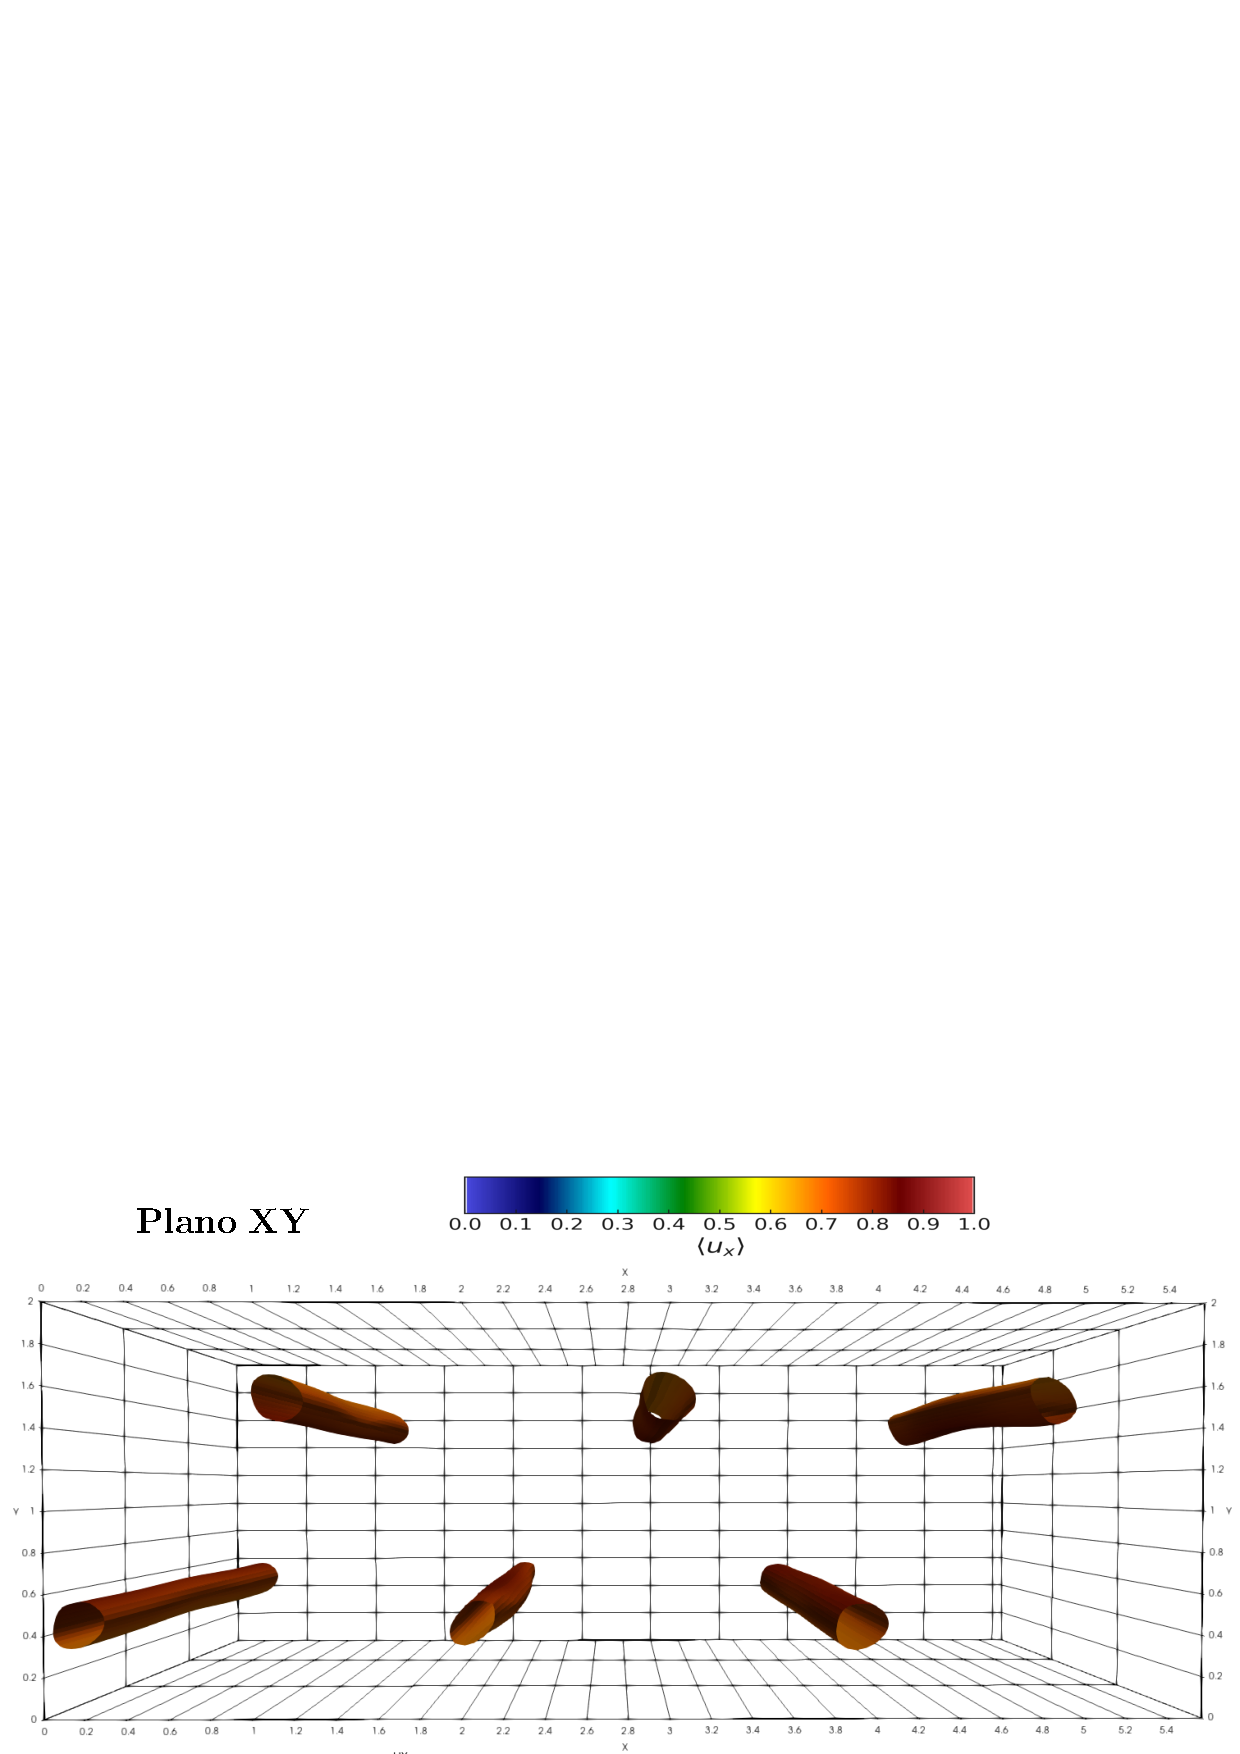
\includegraphics[width=0.49\textwidth]{figures/cap6/A-C10/screenshots_times/t186_xy.png}
    \label{fig:t186-xy-ac10}}  
  \subfloat[]{
    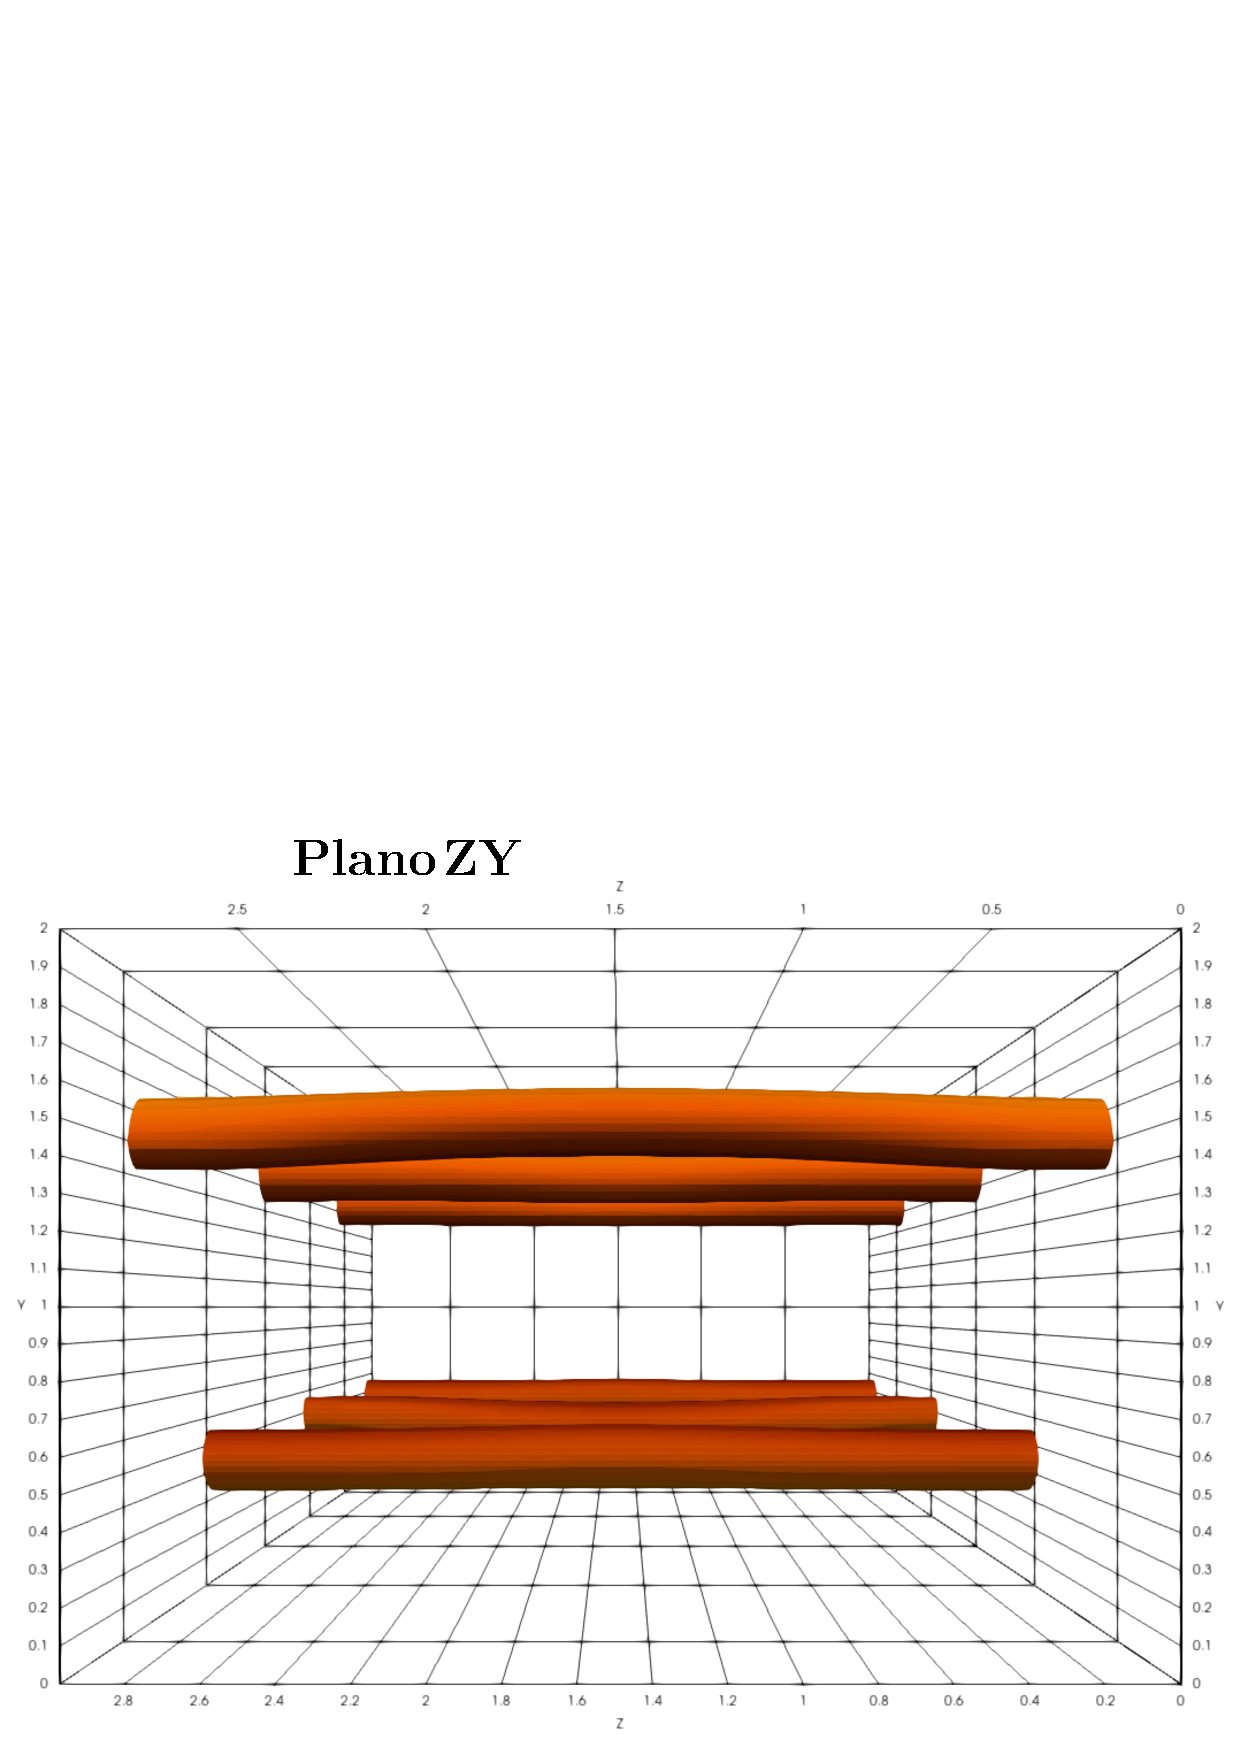
\includegraphics[width=0.49\textwidth]{figures/cap6/A-C10/screenshots_times/t186_zy.png}
    \label{fig:t186-zy-ac10}}
    
  \subfloat[]{  
    \includegraphics[width=0.49\textwidth]{figures/cap6/A-C10/screenshots_times/t338_xy.png}
    \label{fig:t338-xy-ac10}}  
  \subfloat[]{
    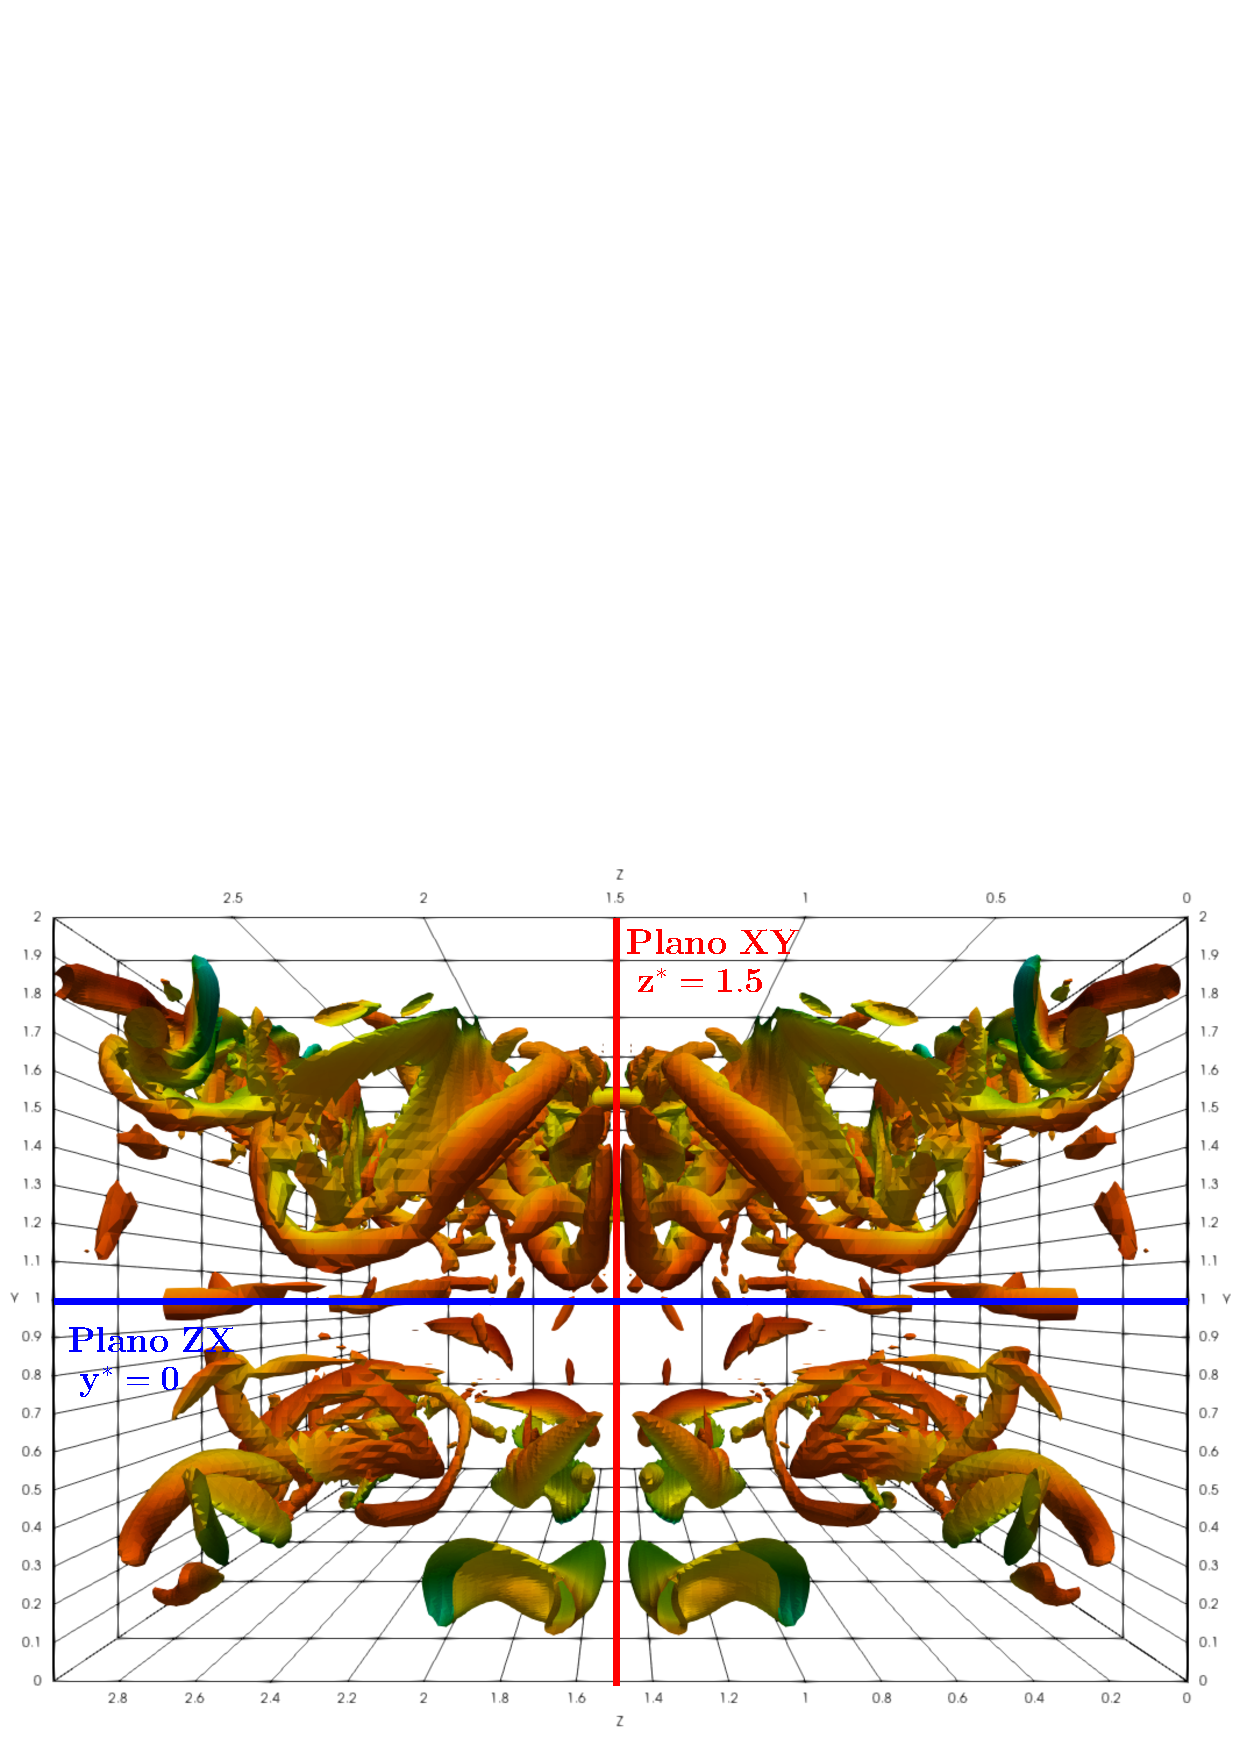
\includegraphics[width=0.49\textwidth]{figures/cap6/A-C10/screenshots_times/t338_zy.png}
    \label{fig:t338-zy-ac10}}
  
  \subfloat[]{ 
    \includegraphics[width=0.49\textwidth]{figures/cap6/A-C10/screenshots_times/t1500_xy.png}
    \label{fig:t1500-xy-ac10}}  
  \subfloat[]{
    \includegraphics[width=0.49\textwidth]{figures/cap6/A-C10/screenshots_times/t1500_zy.png}
    \label{fig:t1500-zy-ac10}}
  \caption{Ensayo A-C10. Capturas de las estructuras de vórtices para tres instantes de tiempo: $t^* =186$ con $Q=0\text{.}1$ (\textbf{(a)} y \textbf{(b)}), $t^* =338$ con $Q=0\text{.}5$ (\textbf{(c)} y \textbf{(d)}) y $t^* = 1500$ con $Q=0\text{.}5$ (\textbf{(e)} y \textbf{(f)}). Aquí $Q$ hace referencia al parámetro del Criterio Q.}
  \label{fig:mosaico2-ac10}
\end{figure}


\subsection{Factor de fricción de Darcy y número de Nusselt}
En la Figura \ref{fig:darcy-ac10} se presenta la evolución temporal del factor de fricción de Darcy. En la \textbf{Zona I} (0 < $t^*$ < 150), $f$ permanece prácticamente constante y coincide con el valor inicial/laminar\footnote{Recuérdese que los valores de $f$ y de $Nu$ obtenidos a partir de la solución laminar y de la condición inicial resultan equivalentes.} (línea a trazos azul). En las \textbf{Zonas II y III}, y parte de la \textbf{Zona IV} ($150 \lesssim t^* \lesssim 352 $), se observa primero una disminución suave hasta un mínimo de $f=0\text{.}0167$ en $t^*\approx270$, seguida de un incremento pronunciado que alcanza su máximo en $t^*\approx352$ ($f \approx 0\text{.}037$). A partir de ese pico, y en el resto de la \textbf{Zona IV} ( $t^*\gtrsim352$), $f$ desciende y se estabiliza entre los valores 0.0275 y 0.033, próximo al valor de referencia del caso completamente desarrollado (línea a trazos negra). De esta forma, es posible distinguir con claridad la etapa transitoria y el posterior establecimiento de un régimen turbulento que persiste en el tiempo.

Por último, la Figura \ref{fig:nu-ac10} presenta la evolución temporal del número de Nusselt. El valor se mantiene prácticamente constante y coincidente con la solución laminar hasta $t^* \approx 300$. A partir de allí, crece de manera monótona hasta el final de la simulación. La tendencia apunta claramente al valor del caso turbulento completamente desarrollado en convección mixta; sin embargo, el tiempo físico simulado no resulta suficiente para garantizar la convergencia. Esta misma situación puede observarse en la varianza de la temperatura y en el perfil de temperatura para $t^*=1500$ aunque no de manera tan marcada como en el caso de Nu. Esto sugiere que se requiere extender la simulación para que las magnitudes térmicas alcancen su estado estadísticamente estacionario.

\begin{figure}[H]
  \centering  
  \subfloat[]{
    \includegraphics[width=0.9\textwidth]{figures/cap6/A-C10/Cases_Comp_darcy.png}
    \label{fig:darcy-ac10}}
    
  \subfloat[]{
    \includegraphics[width=0.9\textwidth]{figures/cap6/A-C10/Cases_Comp_nussel.png}
    \label{fig:nu-ac10}}
  \caption{Evolución temporal de \textbf{(a)} factor de fricción de Darcy y \textbf{(b)} número de Nusselt, para el caso A-C10.}
  \label{fig:ac10-1}
\end{figure}



\newpage
\section{Análisis detallado del caso B‑C2} \label{sec:bc2}

\subsection{TKE y varianza de la temperatura adimensional}
En las Figuras \ref{fig:tke-bc2} y \ref{fig:tetavar-bc2} se expone, respectivamente, la evolución temporal de la energía cinética turbulenta (TKE) y la varianza de la temperatura; dicha evolución se separa en tres regiones. Se añaden valores constantes de referencia asociados al cálculo de dichas cantidades empleando la condición inicial y el flujo turbulento en estado estadísticamente estacionario.

\begin{itemize}

  \item \textbf{Zona I ($0 \lesssim \mathbf{t^*} \lesssim 32$).} Ambas cantidades se mantienen prácticamente constante y coinciden con su valor de referencia asociado a la condición inicial. El sistema no transiciona.

  \item \textbf{Zona II ($32 \lesssim \mathbf{t^*} \lesssim 100$).} Aquí, la TKE crece y alcanza un máximo absoluto en $t^* \approx 46$ ($k_{\text{max}}$ $\approx 0\text{.}134$), superando en dos órdenes de magnitud al valor registrado en el ensayo A-C10. De forma similar, la varianza de la temperatura crece hasta que alcanza un máximo absoluto en el mismo instante de tiempo que la TKE, con un valor $\langle \theta^{*\prime} \theta^{*\prime}\rangle_{\text{max}} \approx 8700$, siendo casi un orden de magnitud menor que en el ensayo A-C10. A partir de $t^* \approx 46$, ambas magnitudes decrecen sin retornar a los valores iniciales, y tienden hacia el estado estadísticamente estacionario del flujo turbulento correspondiente.

  \item \textbf{Zona III ($\mathbf{t^*} \gtrsim 100$).} En esta etapa, ambas magnitudes fluctúan entorno a las magnitudes constantes de referencia: la TKE se mantiene acotada entre 0.002 y 0.005, mientras que la varianza de la temperatura se encuentra entre 0.05 y 0.06. Hacia el final de la simulación, el sistema tiende hacia un nuevo estado de flujo, es decir, uno turbulento. 

\end{itemize}


\begin{figure}[H]
  \centering  
  \subfloat[]{
    \includegraphics[width=0.9\textwidth]{figures/cap6/B-C2/Cases_Comp_tke.png}
    \label{fig:tke-bc2}}
    
  \subfloat[]{
    \includegraphics[width=0.9\textwidth]{figures/cap6/B-C2/Cases_Comp_tetavar.png}
    \label{fig:tetavar-bc2}}
  \caption{Evolución temporal de \textbf{(a)} la energía cinética turbulenta y \textbf{(b)} la varianza de la temperatura, para el caso B-C2.}
  \label{fig:bc2-2}
\end{figure}

\subsection{Perfiles de velocidad y temperatura}
En las Figuras \ref{fig:uxs-bc2} y \ref{fig:phis-bc2} se presentan, respectivamente, los perfiles de velocidad y de temperatura adimensional para $t^*$ = 2, 46, 160, 500, 1000 (de izquierda a derecha). Como referencia, se incluye el perfil correspondiente al flujo completamente desarrollado en convección mixta. La selección de tiempos abarca el régimen laminar inicial ($t^* = 2$), el máximo absoluto en $t^* \simeq 46$, el máximo local subsiguiente de mucho menor intensidad, en $t^* \simeq 160$, y dos instantes posteriores en los que el flujo ya se encuentra en régimen turbulento.

En la etapa inicial, el perfil exhibe la simetría característica de la solución laminar en forma de ``M''. Entorno al máximo absoluto de la TKE, los perfiles se ensanchan levemente y muestran, nuevamente, una aparente pérdida de simetría. Asimismo, el valor de la pendiente en las paredes se incrementa ligeramente en ambas magnitudes, siendo este cambio casi imperceptible en el perfil de velocidad y más notorio en el perfil de temperatura. A medida que aumenta el tiempo, los perfiles de ambas magnitudes convergen hacia las soluciones de referencia del flujo completamente desarrollado. En comparación con el caso A-C10, el aumento de la fuerza boyante tiene por efecto acelerar la evolución del campo de temperaturas, favoreciendo una convergencia más rápida hacia el flujo completamente desarrollado.

\begin{figure}[H]
  \centering  
  \subfloat[]{
    \includegraphics[width=1.02\textwidth]{figures/cap6/B-C2/ux_profiles_mosaic.png}
    \label{fig:uxs-bc2}}
  
  \subfloat[]{
    \includegraphics[width=1.02\textwidth]{figures/cap6/B-C2/phi_profiles_mosaic.png}
    \label{fig:phis-bc2}}
  \caption{Perfiles de \textbf{(a)} velocidad y \textbf{(b)} temperatura adimensional para distintos instantes $t^*$ correspondiente al caso B-C2.}
    \label{fig:mosaico-bc2}
\end{figure}


Nuevamente se analizan las estructuras de vórtices, mediante un enfoque cualitativo, con la intención de entender la aparente pérdida de simetría en los perfiles que ocurre en $t^* = 46$. En la Figura \ref{fig:mosaico2-bc2} se exponen capturas de las isosuperficies asociadas para tres tiempos distintos: $t^* = 2$ (Figuras \ref{fig:t2-xy-bc2} y  \ref{fig:t2-zy-bc2}),  $t^* = 46$  (Figuras \ref{fig:t46-xy-bc2} y \ref{fig:t46-zy-bc2}) y  $t^* = 500$  (Figuras \ref{fig:t500-xy-bc2} y \ref{fig:t500-zy-bc2}). Obsérvese que las capturas ubicadas a la derecha corresponden a la vista del dominio desde un punto de vista normal a los planos $XY$, mientras que las ubicadas a la izquierda muestran la vista normal a los planos $ZY$.

En el instante $t^* = 2$, se observa una estructura coherente y ordenada, asociada las ondas TS. Esto es consistente con la simetría de los que perfiles en la condición inicial; asimismo, dichas estructuras se posicionan muy cercana de las pared al igual que ocurre con los máximos del perfil de velocidad.

En el segundo tiempo considerado, se observa la ausencia total de cualquier estructura coherente; en este punto, la turbulencia producida ha disipado las estructuras de mayor tamaño que pudiesen haberse originado en instantes previos. Asimismo, pareciera que las estructuras no se aglomeran de forma simétrica respecto a las paredes ($y^*=\pm 1$). Una visualización más clara, se aprecia en las Figuras \ref{fig:t46-xy2-bc2} y \ref{fig:t46-zy2-bc2} donde se muestran cortes de planos $XY$ y $ZY$, en $z^* = L_z/2 = 2\text{.}8$ y $x^* = L_x / 2 = 3\text{.}14$, respectivamente. Este ``desequilibrio'' de pequeñas estructuras produce una mezcla no homogénea de las cantidades, lo que podría dar cierto entendimiento, al menos conceptual, del hecho que los máximo del perfil de velocidad cerca las paredes sea distinto.   

Por su parte, en el último instante de tiempo considerado (estado estadísticamente estacionario), se aprecia que estructuras de mayor tamaño han vuelto a resurgir y también carecen de coherencia y orden. Asimismo, viendo la coloración de las estructuras, se puede apreciar que la velocidad \textit{streamwise} a lo largo de la dirección $Y$ es homogénea, salvo en las paredes donde es mayor. Esto resulta consistente con lo observado en el perfil de velocidad \textit{streamwise} (Figura \ref{fig:uxs-bc2}).

Resulta evidente que el efecto de la fuerza boyante impacta considerablemente en como el fluido evoluciona en el tiempo. Uno de los efectos más notables, como se menciona anterioremente, es la aceleración de la dinámica del sistema; esta se traduce en una convergencia al estado turbulento completamente desarrollado en menor tiempo.  


\begin{figure} %[H]
  \centering  
  \subfloat[]{
    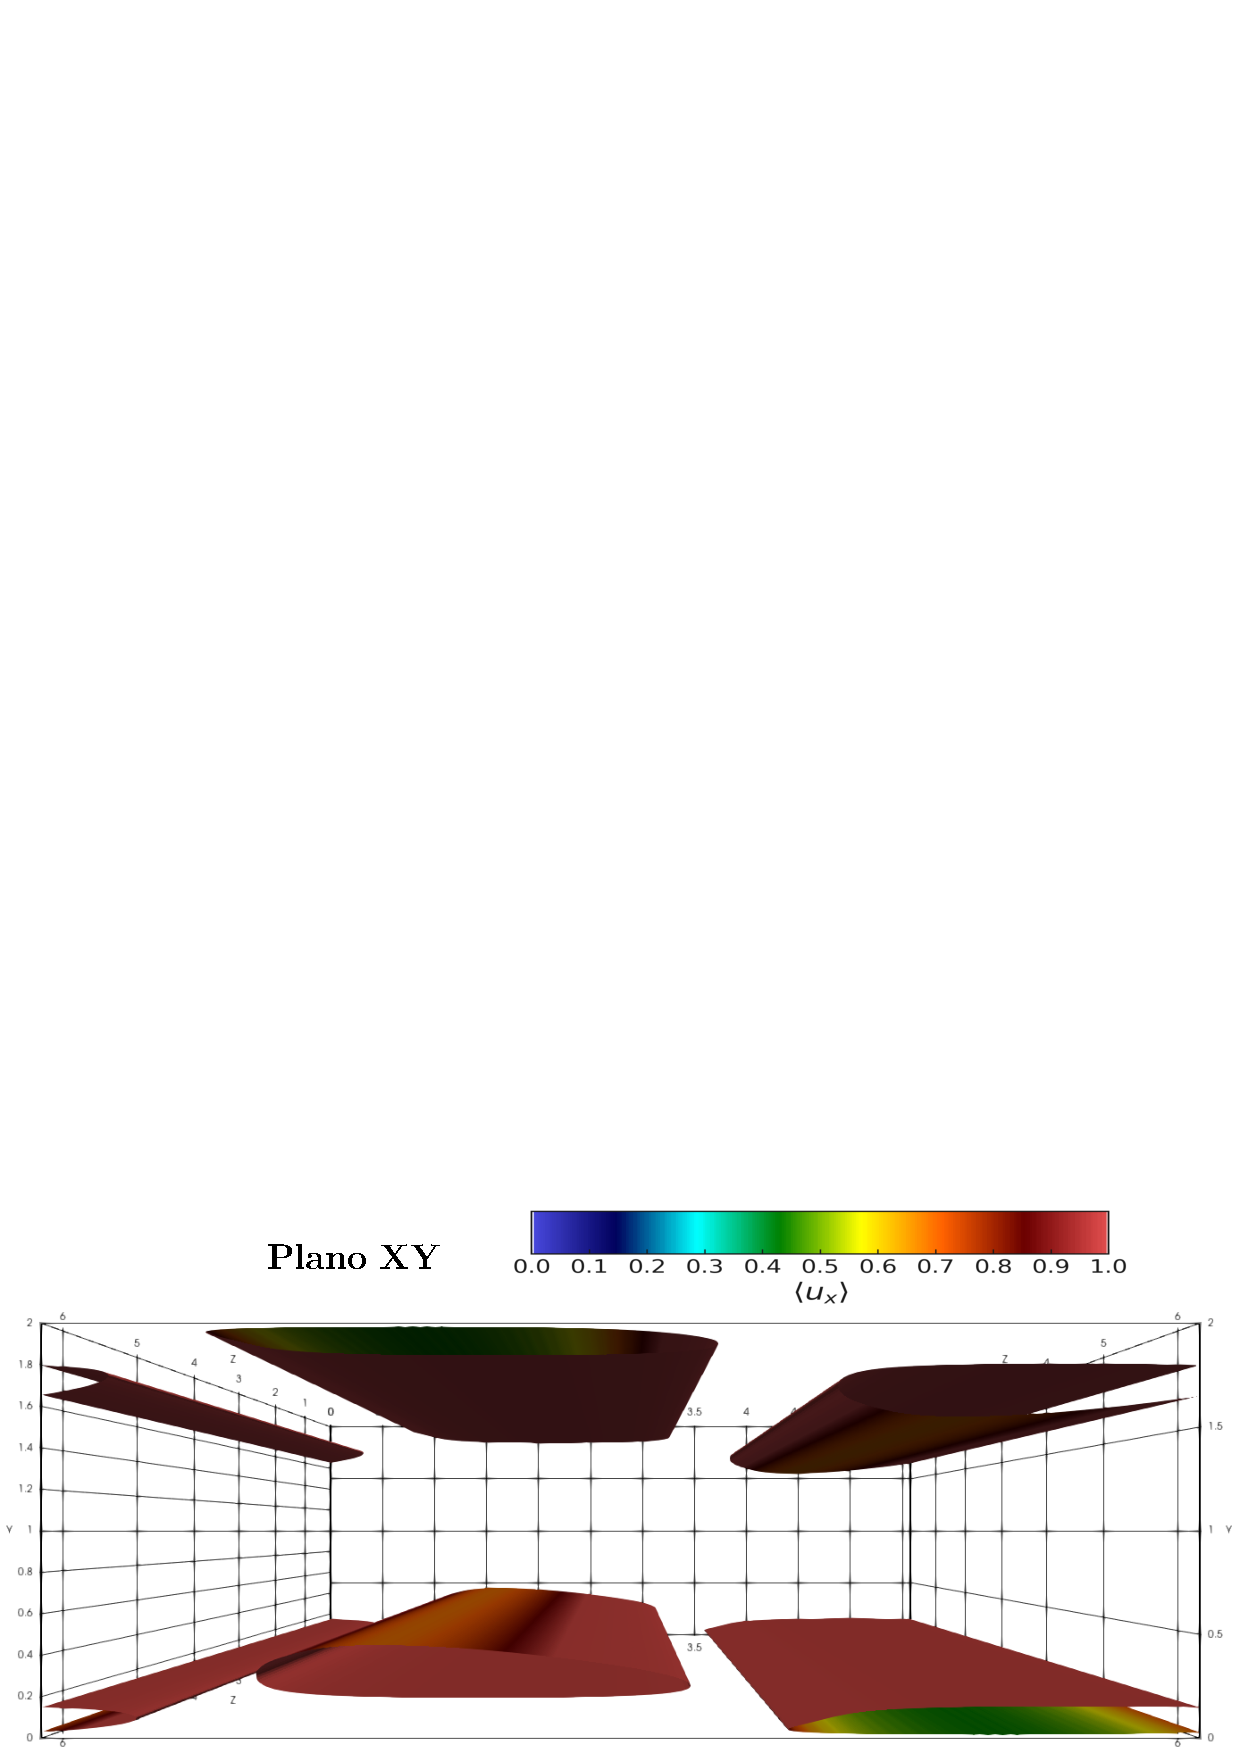
\includegraphics[width=0.49\textwidth]{figures/cap6/B-C2/screenshots_times/t2_xy.png}
    \label{fig:t2-xy-bc2}}  
  \subfloat[]{
    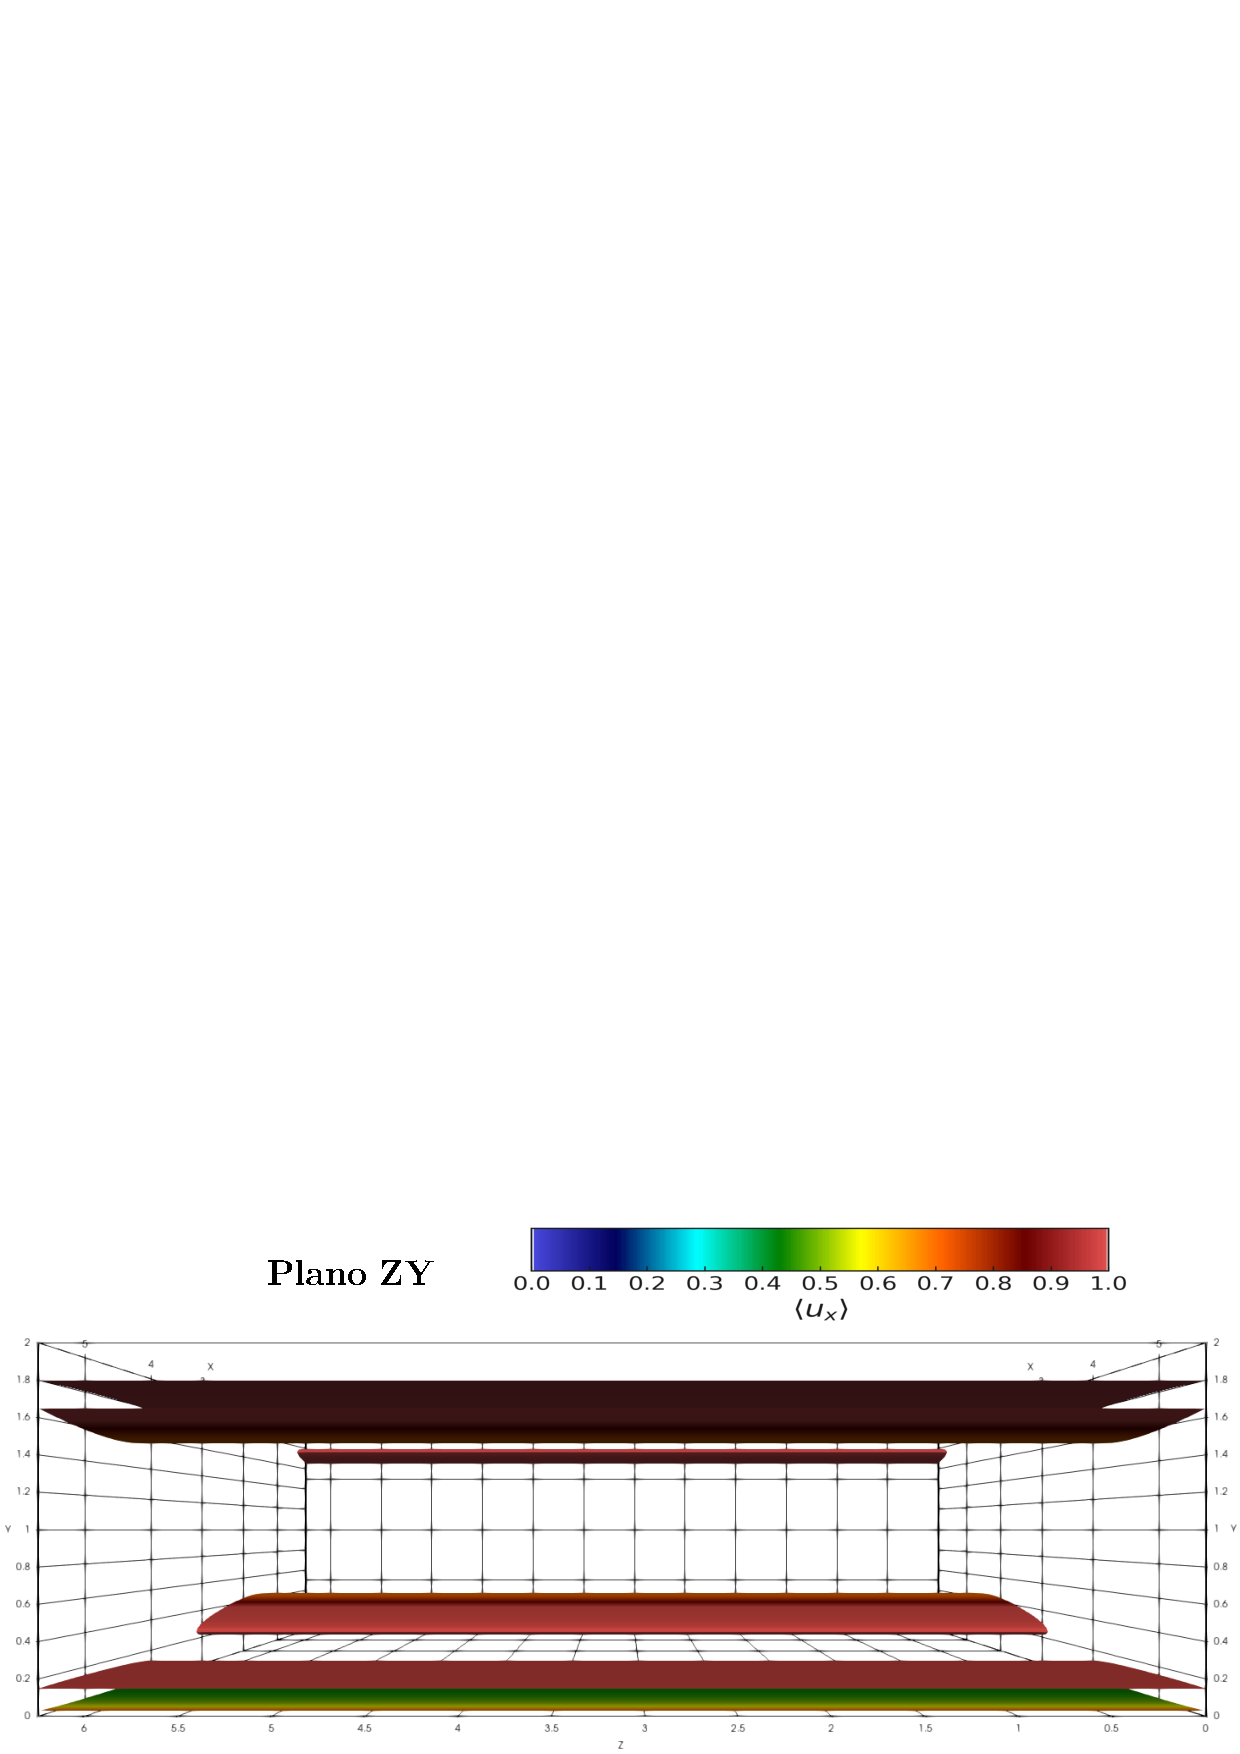
\includegraphics[width=0.49\textwidth]{figures/cap6/B-C2/screenshots_times/t2_zy.png}
    \label{fig:t2-zy-bc2}}
    
  \subfloat[]{
    \includegraphics[width=0.49\textwidth]{figures/cap6/B-C2/screenshots_times/t46_xy.png}
    \label{fig:t46-xy-bc2}}  
  \subfloat[]{
    \includegraphics[width=0.49\textwidth]{figures/cap6/B-C2/screenshots_times/t46_zy.png}
    \label{fig:t46-zy-bc2}}

  
  \subfloat[]{
    \includegraphics[width=0.49\textwidth]{figures/cap6/B-C2/screenshots_times/t500_xy.png}
    \label{fig:t500-xy-bc2}}  
  \subfloat[]{
    \includegraphics[width=0.49\textwidth]{figures/cap6/B-C2/screenshots_times/t500_zy.png}
    \label{fig:t500-zy-bc2}}
  \caption{Ensayo B-C2. Capturas de las estructuras de vórtices para tres instantes de tiempo: $t^* =2$ con $Q=0\text{.}0005$ (\textbf{(a)} y \textbf{(b)}), $t^* =46$ con $Q=10$ (\textbf{(c)} y \textbf{(d)}) y $t^* = 500$ con $Q=0\text{.}4$ (\textbf{(e)} y \textbf{(f)}). Aquí $Q$ también hace referencia al parámetro del Criterio Q. }
  \label{fig:mosaico2-bc2}
\end{figure}

\begin{figure} %[H]
  \centering  
  \subfloat[]{
    \includegraphics[width=0.49\textwidth]{figures/cap6/B-C2/screenshots_times/t46_xy2.png}
    \label{fig:t46-xy2-bc2}}  
  \subfloat[]{
    \includegraphics[width=0.49\textwidth]{figures/cap6/B-C2/screenshots_times/t46_zy2.png}
    \label{fig:t46-zy2-bc2}}

  \caption{Ensayo B-C2. Cortes de las isosuperficies correspondientes al instante $t^* =46$: \textbf{(a)} plano $ZY$ en $x^*=3\text{.14}$ y \textbf{(b)} plano $XY$ en $z^*=2\text{.8}$.}
  \label{fig:mosaico3-bc2}
\end{figure}




\subsection{Factor de fricción de Darcy y número de Nusselt}
La Figura \ref{fig:darcy-bc2} muestra la evolución temporal del factor de fricción de Darcy. En las \textbf{Zonas I y II}, desde el inicio hasta $t^* \approx 20$, $f$ se mantiene próximo al valor laminar (línea a trazos azul). Entre $t^* \approx 20$ y $t^* \approx 46$ el factor de fricción experimenta dos picos sucesivos antes de culminar en un máximo absoluto, $f_{\max}$ $\approx$ 0.174; a partir de ese punto, $f$ decrece de manera pronunciada por debajo del valor laminar inicial. En la \textbf{Zona III}, la curva permanece entorno al valor de la referencia del flujo completamente desarrollado hasta $t^* \approx 400$; luego, la magnitud adquiere valores por debajo del valor de referencia antes mencionado. Si bien estos valores estan cercanos al valor de referencia, son claramente distinto a él. Esto último no es necesariamente una señal de que el resultado converge a un valor diferente, sino más bien una pista que posiblemente el sistema requiera más tiempo para desarrollarse. 

Por su parte, la Figura \ref{fig:nu-bc2} muestra la evolución temporal de Nu. Se observa que el número de Nusselt se mantiene cercano a la solución laminar inicial hasta $t^* \approx 34$, luego comienza a decrecer hasta un valor mínimo en $t^* \approx 48$ ($\text{Nu}_{\text{min}} \simeq 10\text{.}6$). A partir de allí, Nu comienza un período de crecimiento de manera monótona y sostenida, superando el valor inicial de referencia, tendiendo a la referencia del estado estadísticamente estacionario. El valor mínimo que alcanza Nu, coincide aproximadamente con el instante donde TKE es máximo. \textcolor{blue}{La TKE nos da una idea de la turbulencia producida por el flujo, por lo cuál, podría considerarse que para ese instante el calor se distribuye de la forma mas homogénea posible produciendo el aumento máximo de la temperatura bulk (ecuación \ref{eq:nu}) y por lo tanto el mínimo de Nu.}  

\textcolor{red}{NOTA PARA DIRECTORES: Dado la definición que use de Nu en el Cap 5 \ref{eq:nu}, no puedo sacar nada útil de los perfiles para explicar el mínimo de Nu. Lo intenté pero queda inconsistente y no cierra (Willi me lo marcó). Por otro lado poner la evolución temporal de $\langle \theta_b \rangle$ no dice nada ya que es como la curva de Nu pero espejada respecto al eje horizonal; ese comportamiento es medio obvio y se entiende si uno mira la evolución  temporal  del Nu y tiene en cuenta que Nu $\propto 1/\langle \theta_b \rangle$. Intenté darle una explicación con el tema de la producción de la turbulencia, la mezcla homogenea de las cantidades y el aumento de la temperatura dimensional pero no creo que esté bien.}


%El decrecimiento y posterior ascenso del número de Nusselt en la región $34 \lesssim t^* \lesssim 120 $ puede entenderse cualitativamente a partir de la estructura de vórtices. La cantidad de vórtices en $t^* \approx 46$ (Figura \ref{fig:t46-xy-bc2}) muestra que el grado de turbulencia es tan grande que da lugar a una muestra 

%El decrecimiento y posterior crecimiento de Nu para $34 \lesssim t^* \lesssim 120 $ puede entenderse en términos de la derivada de la temperatura en las paredes. Utilizando la definición de Nu, el hecho de que $q''_w = h \langle \theta_b \rangle$ y que $q''_w = \kappa \frac{dT}{dy}$ (en $y=\pm d$), el mismo puede reescribirse como se muestra en la ecuación \ref{eq:nu2}. El valor de la temperatura bulk se mantiene practicamente constante para $t^*=2,46,160$ ($\langle \theta_b^* \rangle \approx 0\text{.}002$). Además, tengase en cuenta que $dT/dy = - d \theta /dy$ por lo que si $d \theta /dy$ aumenta cerca de las paredes, entonces  $dT /dy$ decrece en las paredes. Empleando lo mencionado anteriormente, y observando los perfiles de temperatura adimensional, resulta claro que $d T /dy$ disminuye para $t^*=46$ respecto a su valor en $t^*=2\text{, }160$; por lo tanto, Nu disminuye en $t^*=46$ siendo mayor en los instantes $t^*=2\text{, }160$.
%
%\begin{equation}
%\begin{aligned}
%\text{Nu} = \frac{h d}{\kappa} = \frac{q''_w d}{\langle \theta_b \rangle} \left.\frac{dT}{dy}\right\vert_{w}
%\end{aligned}
%\label{eq:nu2}
%\end{equation}

\begin{figure}[H]
  \centering  
  \subfloat[]{
    \includegraphics[width=0.9\textwidth]{figures/cap6/B-C2/Cases_Comp_darcy.png}
    \label{fig:darcy-bc2}}
    
  \subfloat[]{
    \includegraphics[width=0.9\textwidth]{figures/cap6/B-C2/Cases_Comp_nussel.png}
    \label{fig:nu-bc2}}
  \caption{Evolución temporal de \textbf{(a)} factor de fricción de Darcy y \textbf{(b)} número de Nusselt, para el caso B-C2.}
  \label{fig:bc2-1}
\end{figure}

\section{Comparación: A-C10 vs B-C2}

A continuación se realiza una breve comparación entre los dos casos analizados en mayor detalle. En primer lugar, para el ensayo A-C10 (Ri$_b$ = 0.04) fue requerido emplear una combinación de ondas bidimensionales y tridimensionales para inducir la inestabilidad del flujo y lograr que transicione. Lo contrario ocurre en el ensayo B-C2 (Ri$_b$ = 1.06) donde bastó con utilizar únicamente una onda bidimensional.

El aumento de la fuerza boyante acelera el desarrollo hidrodinámico y en particular, el desarrollo térmico. Esto queda claro al inspeccionar los perfiles de velocidad y temperatura de ambos ensayos (Figuras \ref{fig:mosaico-ac10} y \ref{fig:mosaico-bc2}). Ademas, cerca de las paredes, los perfiles de ambos casos experimentan un aumento de la pendiente en el instante de tiempo que coincide con el máximo absoluto de la TKE asociada.

Al inpeccionar la energía cinética tubulenta y la varianza de la temperatura, se distingue que en el ensayo A-C10 primero se produce un aumento y descenso de estas magnitudes (dos picos de menor intensidad) antes del crecimiento que da paso al establecimiento del nuevo estado de flujo; sin embargo, en B-C2 no existen aumentos y/o descensos intermedios de las magnitudes sino un crecimiento brusco que ocurre en un instante de tiempo temprano en comparación al ensayo A-C10.

Al inspeccionar el coeficiente de fricción, el ensayo A-C10 inicia con un valor $f$ menor al que luego alcanza en el estado turbulento desarrollado; por su parte, en B-C2 ocurre lo contrario, partiendo de un valor inicial mas alto, este evoluciona y alcanza luego un valor menor cuando se encuentra en el estado estíditicamente estacionario. Asimismo, antes del valor pico mencionado, el coeficiente de fricción experimenta un valle en el ensayo A-C10, sin embargo, en B-C2, la magnitud no experimenta decaimiento alguno. En general, las magnitudes TKE, varianza de la temperatura y factor de fricción evolucionan al estado estadísticamente estacionario experimentando más fluctuaciones en el caso A-C10 respecto al caso B-C2.

Por último, en el ensayo B-C2, el número de Nusselt experimenta una caida brusca para instantes de tiempos cercanos al inicial, algo que no ocurre en el ensayo A-C10. Asimismo, luego de la etapa inicial, en ambos casos el Nu crece de forma monotona, no obstante, en ninguno de los ensayos, el tiempo simulado fue suficiente para que Nu alcanze los valores asociados al estado estíditicamente estacionario.



\section{Sumario de los principales hallazgos}
\begin{itemize}

\item \textbf{Naturaleza de la perturbación.} En el ensayo A-C10 (Ri$_b$=0.04) se requiere una combinación de ondas 2D/3D para desencadenar la transición, mientras que en el ensayo B-C2 (Ri$_b$=1.06) una onda bidimensional resulta suficiente.

\item \textbf{Perfiles de velocidad y temperatura.} En ambos casos se observa que los perfiles arrancan con su forma típica laminar, luego evolucionan hasta un estado, que coincide con el tiempo en que ocurre el máximo de la TKE, en donde ambos perfiles pierden su simetría. Una vez atravesada esa etapa, para tiempos más largos los perfiles convergen al caso turbulento completamente desarrollado.  Se observa que el aumento de la fuerza boyante reduce el tiempo de convergencia. 

\item \textbf{Patrón Temporal de TKE y $\langle\theta^{*\prime}\theta^{*\prime}\rangle$.} El caso de A-C10 experimenta un transición intermedia (dos máximos locales de menor intensidad) antes de llegar al pico que produce la transición hacia el estado estadísticamente estacionario. Los valores asociados a dichos estados se encuentran por arriba del valor laminar en $t^*=0$. En el ensayo B-C2 el sistema experimenta una transición brusca, las cantidades alcanzan el máximo absoluto en menor tiempo ($t^*\approx 46$), y luego convergen al valor de referencia del flujo turbulento desarrollado. Se observa que el aumento de la fuerza boyante acelera dicha dinámica. 

\item \textbf{Patrón temporal en factor de Darcy.} En A-C10, la cantidad evoluciona de un estado inicial y crece hasta alcanzar un pico, luego fluctúa entorno al valor de referencia del caso completamente desarrollado por encima del valor de $f$ en $t^*=0$. En B-C2, tras un período corto laminar, la magnitud experimenta dos picos sucesivos de baja amplitud, llega a un máximo absoluto y luego transiciona hacia el estado estadísticamente desarrollado por debajo del estado inicial.   

\item \textbf{Evolución temporal de Nu.} En A-C10, Nu se mantiene practicamente constante hasta $t^* \approx 300$ y luego crece de forma monótona sostenida. Por su parte, en el caso de B-C2, la magnitud experimenta un mínimo en una etapa inicial, luego se recupera y crece de forma monótona al igual que ensayo anterior. En ambos casos, aunque la tendencia a converger es notable, el tiempo de simulación resulta insuficiente. 

\end{itemize}